\chapter{Implementing Models and Algorithms for a Distributed Cloud Manufacturing Network based on autonomous resources}
\label{chapter4}
\section{Introduction}
This chapter outlines the implementation process of core functionalities in the Scattered Manufacturing framework, known as Scattered Manufacturing, by means of demonstrating the flow of the activities through a complete operations cycle. The first paragraph focuses on the implementation of a Multi-Agent System architecture for managing distributed operations. The second paragraph proposes an implementation of a scheduling and logistics optimization algorithm for a large Additive Manufacturing network.
\section{A Multi-Agent System architecture for managing distributed operations}
\subsection{Introduction}
The new generation of information technology dealing with cloud applications, big data, IoT has led to significant changes in manufacturing. The cloud application service provided manufacturers with cloud-based software and collaboration by moving the processing and management of manufacturing information in the cloud and creating the phenomenon of Cloud Manufacturing \parencite{bo-hu_cloud_2010}\parencite{vincent_wang_interoperable_2013}. \textcite{xu_cloud_2012} defines Cloud Manufacturing as “a model for enabling ubiquitous, convenient, on-demand network access to a shared pool of configurable manufacturing resources (e.g., manufacturing software tools, manufacturing equipment, and manufacturing capabilities) that can be rapidly provisioned and released with minimal management effort or service provider interaction”.\\
Cloud Manufacturing aims at sharing and distributing in a collaborative manner large-scale manufacturing resources \parencite{liu_workload-based_2017}. This is possible through a cloud manufacturing platform, which integrates distributed manufacturing resources, transforms them into manufacturing services, and manages them centrally \parencite{adamson_cloud_2015}\parencite{xu_cloud_2012}. Cloud Manufacturing can handle multiple users’ service requests, dealing with multiple manufacturing tasks (manufacturing lot) in parallel. Cloud Manufacturing can manage many distributed and idle manufacturing resources, providing a sustainable, cleaner production \parencite{zhang_analytical_2017}. Anyway, there is no single standard for a Cloud Manufacturing implementation: there are several different Cloud Manufacturing architectures (e.g., see \textcite{bo-hu_cloud_2010}\textcite{liu_workload-based_2017}\textcite{liu_cyber-physical_2017}). The shared resources in Cloud Manufacturing include the computing resource in cloud computing and other manufacturing resources. Such resources include hard manufacturing resources (e.g., machine tools), soft manufacturing resources (e.g., models and a massive amount of data), and manufacturing capabilities (design, production, and test capabilities). The on-demand supply method in cloud computing cannot be directly applied to cloud manufacturing because of some characteristics of manufacturing resources, such as heterogeneity, diversity, and dispersity, which cloud computing does not possess \parencite{he_state---art_2015}. Hence, global scheduling is not always available \parencite{bo-hu_cloud_2010}. In \textcite{ren_cloud_2017}, a 3D printing service (3DPS) scheduling method in the context of Cloud Manufacturing is proposed to generate optimal service scheduling solutions; the method is based on a genetic algorithm. It is clear that one needs to select a suitable service because there may be multiple candidate services for a task. In \textcite{ren_cloud_2017}, four attributes of the 3DPS, including size, material, accuracy, and cost, as the service matching rules, were considered in the scheduling problem. Anyway, in \textcite{ren_cloud_2017}, the dynamic task arrival and downtime of 3D printers were not considered. Besides, the author did not consider anomalous tasks.
In this section, the design of a Multi-Agent System for managing and monitoring 3DPS is proposed, addressing the issues above. Multi-Agent systems \parencite{wooldridge_introduction_2009} represent a technology allowing modularity, flexibility, robustness, and adaptivity in complex systems, and they have been applied in many domains to solve complex problems \parencite{loia_using_2017}\parencite{daniello_multi-agent_2015}\parencite{daniello_self-regulated_2018}. Especially in industrial environments, where some requirements are needed depending on the application scenarios, the design is the first key factor to develop a suitable MAS \parencite{karnouskos_key_2017}.\\
In the following paragraphs, a Multi-Agent System scheme is proposed by analyzing it at the design stage. The analysis is supported by simulating some nodes through a small hardware system to check on communication issues.
\subsection{Problem Formalization}
In this paragraph, we briefly describe the problem and its context. Herein, we consider the Scattered Manufacturing Network [54], an adaptation of a Cloud Manufacturing network architecture described in the previous chapter. In a Scattered Manufacturing network, nodes are autonomous entities able to instance job orders or offer manufacturing services coordinated by an Orchestrator. The Orchestrator is responsible for the negotiation among nodes, ensuring the respect of network policy, and the overall optimization in the Supply Network. Scattered Manufacturing network policy obeys three main principles: sustainability, equally shared resources among nodes, and transparency.\\
Sustainability occurs in cost-effective manufacturing, reducing resource demands and related CO2 emissions over the entire product life cycle, transferring the production closer to the end-user. The Scattered Manufacturing network aims to create a collaborative, transparent, open,, and trusting environment with shared purposes and shared resources \parencite{de_falco_negotiating_2017}. Cloud Manufacturing requires the interaction between three groups: the users, application providers, and physical resource providers \parencite{wu_cloud_2013}. In a Scattered Manufacturing network, actors are grouped and labeled as: Demanding nodes, Orchestrator, Manufacturing nodes. The Orchestrator coordinates resources and workloads matching orders from demanding nodes and local manufacturing available capacity.\\
At the first stage, demanding nodes submit their job orders with the required accuracies and admissible quantities, and cost ranges. The platform then localizes the order to define a subset of candidate manufacturing nodes. Potential resource providers are then filtered, considering technical constraints derived from job requirements.\\
Each service demanders have distinctive priorities in the optimization objective function \parencite{zhou_multi-task_2018}. A weight coefficient represents a priority ri according to the demander’s latest product delivery time. Then we have a minimization problem, which is formulated as follows:\\

\begin{equation}
    \label{eq:1}
    \min{\frac{\sum _i r_i F_i}{\sum _i r_i}}
\end{equation}

where Fi is the product delivery time of a specific service demander Di, and it takes into account the start time of the task, the printing time, and logistics time.\\
The constraints are mostly inequality constraints, such as:
\begin{itemize}
    \item model size, that is the maximum admissible size of the selected \emph{kth} service $S_k$ must not be smaller than the size of the 3DP model of task $t_i$ 
    \begin{equation}
        \label{eq:2}
        \min\left(u_i,v_i\right)\leq\min\left(U_k, V_k\right)
    \end{equation}
    \begin{equation}
        \label{eq:3}
        \max\left(u_i,v_i\right)\leq\max\left(U_k, V_k\right)
    \end{equation}
    \begin{equation}
        \label{eq:4}
        w_i \leq W_k
    \end{equation}
\end{itemize}
where $u_i$, $v_i$, $w_i$ are the length, width, height of the 3D model associated with the task $t_i$, respectively, $U_k$, $V_k$, $W_k$ are the maximum length, the maximum width, the maximum height of machine working area selected for $S_k$ respectively:
\begin{itemize}
    \item printing accuracy: the accuracy $A_k$ of the selected 3DP service $S_k$ should be smaller than the printing accuracy $a_i$ of task $t_i$ \begin{equation}\label{eq:5}A_k \leq a_i \end{equation}
    \item the cost: the acceptable maximum cost $c_i$ of task $t_i$ should be not higher than the practical task completion cost $C_k$ with regard to the selected service $S_k$ \begin{equation}\label{eq:6}c_i \leq C_k \end{equation}
\end{itemize}

and an equality constraint, that is:
\begin{itemize}
    \item printing materials: since the printing material type $M_k$ of the selected 3DP service $S_k$ must be the same as the printing material type of $i_th$ task $m_i$ \begin{equation}\label{eq:6}m_i = M_k \end{equation}
\end{itemize}
The optimization problem can be solved using a genetic algorithm (GA) \parencite{zhou_multi-task_2018}. It is the case to point out that, after the localization and filtering stage, the Orchestrator needs to fragment the order into a finite number of tasks that will be assigned to the resource providers. The assignment phase requires negotiations and optimization steps to obtain an optimal solution. Further details about this topic, as well as numerical approaches, are discussed in
the following paragraphs and have been detailed in \textcite{de_falco_negotiating_2017} and \textcite{de_falco_integrating_2019}.
In order to tackle some issues such as dynamic task arrival and downtime of 3D printers, as well as anomalous tasks, in the next paragraph, a Multi- Agent System scheme handling the optimization problem in a more general way is introduced.
\subsection{The proposed Multi Agent System architecture}
A Multi-Agent System is a system composed of interacting intelligent agents that are autonomous entities that can act and communicate with each other in a certain context, depending on the environment state \parencite{lopes_negotiation_2009}.\\
For each agent a finite set A of actions are possible: \begin{equation} \label{eq:7} A = \left\{A_1,A_2,...,A_n\right\}\end{equation}
Through actions, each agent interacts with the environment. As a consequence, the environment assumes a finite number of possible states: \begin{equation} \label{eq:8} X = \left\{X_1, X_2, ...\right\} \end{equation}
In the proposed model, the objects of monitoring are tasks, printers, scheduling, and the system's fitness. We consider a multi-agent system (MAS) model, with three types of agents: Task Agent (TA), Master Agent (MA), and Printer Agent (PA).\\
The task agent (TA) collects and processes tasks, then organizes them according to the user requirements and provider policy. The TA handles batches of n tasks as follows:
\begin{multline}
    \label{eq:9}
    B=\{t_1,...,t_n,r_1,...,r_n,w_1,...,w_n,o_1,...o_n,a_1,...,a_n,m_1,...,m_n,\\ 
        h_1,...,h_n,c_1,...,c_n,d_1,...,d_n,\mu,\sigma\}
\end{multline}
where:
\begin{itemize}
    \item $t_i$, with i=1,...,n, are the tasks
    \item $r_i$, with i=1,...,n, the priority of the ith task
    \item $w_i$, with i=1,...,n, is the workload for the ith task
    \item $o_i$, with i=1,...,n, is the 3DP output size for the ith task
    \item $a_i$, with i=1,...,n, is the required accuracy for the ith task
    \item $m_i$, with i=1,...,n, is the demanded material for the ith task
    \item $h_i$, with i=1,...,n, hashes of tasks
    \item $c_i$, with i=1,...,n, the acceptable maximum cost for each task given the service demander
    \item $d_i$, with i=1,...,n, delivery location of ith task
    \item $\mu$ mean workload of all scheduled batches
    \item $\sigma$ standard deviation of workload for each scheduled batch
\end{itemize}

The mean $\mu$ and standard deviation $\sigma$  of the workloads are computed to compare the current workload to the ones of past tasks. This evaluation process allows checking if the workload of a task is below a certain threshold as follows:
\begin{equation}
    \label{eq:10}
    |w_i - \mu| < \alpha * \sigma
\end{equation}
where $\alpha$ is a tuning parameter to be determined.
If the workload is over the threshold, tasks return to the service demander. This phase allows realizing a sort of global optimization to ensure a certain balance in the global network of printers to not overload a node or assign only small works to a given node.\\
The TA is also responsible for monitoring tasks by checking task features such as task size and task integrity to perform a local optimization. It is equipped with a classifier, e.g., an Artificial Neural Network (ANN) or a Functional Network \parencite{gaeta_generalized_2013} \parencite{cha_multi-agent_2015} (in case only small datasets are available for the learning), to detect anomalously (not fitting to usual demand) tasks. Indeed, an anomalous task is a task that presents a set of features (e.g., quantity, accuracy, sizes) that have never been seen before. For this anomalous task, the classifier present in the TA agent will label the task as false. This false task will not be immediately rejected but sent back for human confirmation by an operator. As usual, the classifier works in two stages: an offline stage, which is the stage where the ANN learns the tasks from certain users; an online stage, where the training dataset is updated by adding new cases.\\
The training dataset contains a triplet of input attributes for the ith task, that is, workload $w_i$, output size $o_i$, required accuracy $a_i$, and a single desired output, which is a binary value, that is 0 or 1, representing the false or true task. During the online stage, each task detected as “false” is sent back to the user for additional confirmation. If the user confirms the task as a “true task”, then it is added a new sampling pattern to the dataset.\\
Printer agents (PAs) monitor if a particular printer is under or overloaded. A PA records the downtime of the printer. Then, if the idle time is below a given threshold $\tau_0$ it communicates to the master agent (MA) that the printer is overloaded and it needs less work to operate; if the idle time is above a threshold $\tau_v$, then it communicates that it is underloaded and, in this case, the PA communicates its own cost for the task.\\
PAs are also in charge of checking task integrity before the execution. The task body is hashed, and this hash is then compared with the hash provided by MA. If the hashes are the same, the task is processed. If not, it means that the task was modified and in such a case the task is uploaded from MA again.\\
A master agent checks all basic system characteristics: it is responsible for generating times of starting task scheduling, as well as monitoring and supporting the genetic process of scheduling. When the schedule is ready, tasks are disposed to the printer units to be executed. During task execution, MA gathers the information from PA. Then it decides if the workload should be increased or decreased to obtain optimal printer utilization. This is measured by the assumed fitness function of the system. The fitness of the system depends on the printers’ utilization. They may be idle or overloaded. If many printers are idle, then MA makes a decision about scheduling forcing, and dispatching a new portion of tasks. The decision is made on the basis of a social behavior model involving the PAs. We adopt a hybrid voting scheme.\\
If more than a threshold $p$ of the PAs is reporting that less work is required, the batches are sent q\% less frequently. If more than p of the PAs are reporting that more work is required and the total cost associated with such PAs is not higher than $c$, the batches are sent q\% more frequently. The parameters $p$ and $c$ are set in a proper way.
The actions of the agents may be described in pseudocode in what follows. The signature of each algorithm indicates the agent's name (e.g., TA: meansTask Agent:); followed by the name of the action with its parameters. Different agents may execute the same action but with different behavior. The basic behavior that emerges by the cooperation between the agents is the following: 1) the Task Agent (TA) checks the data received by the service demander (Listing 1). This input data represents the batch B of n tasks in equation \ref{eq:9}. If the information is correct, it sends the request to the Master Agent (MA) (Listing 2). The MA receives this batch B and asks for information to a set of PA regarding $\tau_0$ and $\tau_v$. Once received this information (PA sends the information using the action in Listing 4), MA starts the scheduling. The scheduling consists of creating a set of work queue $Q_j$, each containing a subset of the tasks of batch $B$, and assigning this queue to one of the PA. Therefore, using the scheduling results, MA will send a work queue $Q_j$, together with the hashes $H_j$ of those tasks, to one of the identified $PA_j$ (Listing 3) until all the tasks are assigned. In case one of the PA finds an anomaly or an error, it sends the task back to the MA (Listing 5). In this case, the MA proposes a new scheduling plan (Listing 6).
\begin{algorithm}
    \caption{Task Agent checks the input data received by the service demander.}
    \label{listing1}
    \begin{algorithmic}[1]
        \Procedure{TA: Action\_check(input data)}{}
        \State Receive data from service demander;
        \If
            {task is true} \Return {call Action\_Send(B)}
        \Else { send back to service demander};
        \EndIf
        \EndProcedure
    \end{algorithmic} 
\end{algorithm}

\begin{algorithm}
    \caption{Task agent sends the batch to the Master Agent.}
    \label{listing2}
    \begin{algorithmic}[1]
        \Procedure{TA: Action\_Send(B)}{}
        \State Create the batch B;
        \For {workload in B}
            \If
                {$workload > threshold$} \Return {remove task from B;} {send task to service demander;}
            \EndIf
        \EndFor
        \State Send B to MA;
        \EndProcedure
    \end{algorithmic} 
\end{algorithm}

\begin{algorithm}
    \caption{Master agent receives the information from PAs, perform the scheduling algorithm and sends the work queue Qj (containing the tasks assigned to PAj) and the hashes Hj of the tasks to each PAj identified by the scheduler.}
    \label{listing3}
    \begin{algorithmic}[1]
        \Procedure{MA: Action\_Send(Qj,Hj)}{}
        \State receive resource information from PAs;
        \State call Scheduling;
        \State send $Q_j,H_j$ to $PA_j$;
        \EndProcedure
    \end{algorithmic} 
\end{algorithm}

\begin{algorithm}
    \caption{PA sends the information regarding $\tau_0$ Agent MA.}[1]
    \label{listing4}
    \begin{algorithmic}
        \Procedure{PA: Action\_check($\tau$)}{}
        \If {idle time $\tau$ < $\tau_0$} 
            \Return sent $\tau_0$ to MA;
        \ElsIf {  idle time $\tau$ > $\tau_v$}
            \Return send $\tau_v$ to MA;
        \EndIf
        \EndProcedure
    \end{algorithmic} 
\end{algorithm}

\begin{algorithm}
    \caption{In case of anomalies or errors, PAi sends the task back to the Master Agent MA.}
    \label{listing5}
    \begin{algorithmic}[1]
        \Procedure{PAi: Action\_Send(E)}{}
        \If {$h_i^TA \neq h_i^PA$};
            \Return E=1;
        \EndIf
        \State send E to MA; 
        \EndProcedure
    \end{algorithmic} 
\end{algorithm}

\begin{algorithm}
    \caption{n case a node is not available, MA proposes a new scheduling plan.}
    \label{listing6}
    \begin{algorithmic}[1]
        \Procedure{MA: Action\_Send($Q_j\prime$,$H_j\prime$)}{}
        \If {$\frac{\sum_i \tau^i_v}{\tau_v} > p$ AND $\sum_i c^i < c$};
            \Return call Scheduling;
        \EndIf
        \State send new vectors $Q_j\prime$, $H_j\prime$, to $PA_j$; 
        \EndProcedure
    \end{algorithmic} 
\end{algorithm}

\subsection{Design analysis of the proposed MAS}
Sequence diagrams at the design stage are a visualization tool to sketch inter-agent communications. Figure 15, Figure 16, and Figure 17 show the sequence diagrams referred to three different scenarios.\\
As shown in Figure 15, the process starts when TA sends the batch file B to MA. This behavior is implemented in Listing \ref{listing1} and Listing \ref{listing2}. MA sends a flag R to the printer agents $PA_i$ requesting information on resources (Listing \ref{listing3}). The printer agents PAi respond by sending the idle time $\tau$ and the costs C (Listing \ref{listing4}). According to this information, MA performs the scheduling by sending to PAi the work queue Qi and the hashes of tasks Hi. (Listing \ref{listing3})\\
Figure 16 depicts the case when a new scheduling plan is generated after the printer agents send the parameter $\tau_u$ and the new costs C. In Figure 17, the case when a hash check failed on a PA. Then that PA sends a message error E to MA (Listing\ref{listing5}), which sends again the work queue and the hashes of tasks (Listing \ref{listing6}).\\
As a first check on communication issues, an implementation on a small hardware system, in a certain sense motivated by the ideas inspiring the hardware-in-the-loop simulation, was conducted (e.g., see \textcite{cha_multi-agent_2015}). An Arduino UNO was used in order to simulate the exchange of information between the node MA and a PA node. The MA was simulated using Matlab, providing a suitable function to solve the optimization problem, which is handled by MA.\\
The PA was simulated using Arduino with an ATMEGA328 microcontroller linked to the PC through the serial port. Middleware in the form of a shared folder as a common workspace for Matlab and Arduino was provided. A Java code allowed the simulated nodes to create and to read .txt files. The file name contains the timestamp and the name of the node.\\
The process starts with a .txt file created by MA, simulated by Matlab. Arduino, which simulates PA, will elaborate the file's content by generating a new .txt file. The simulated MA will read the latter by checking it and, in the absence of reading errors, generating a new .txt file.\\
As a result, at the end of the simulation, we found a total delay equal to 0.1 s, mainly due to the elaboration, but not to the communication, with a 1\% rate of reading errors.

\begin{figure}[h]
    \centering
    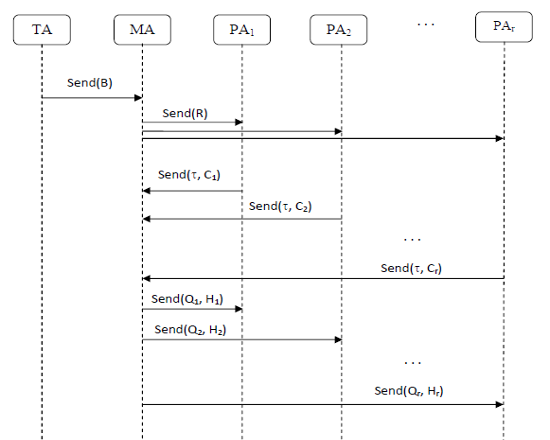
\includegraphics[height=8cm, keepaspectratio]{images/sequence-diagram-case1}
    \caption{Sequence diagram, case 1 – starting the process (B = batch file; Qi= work queue; Hi= hashes of tasks; R= flag for requesting information on resources)}
    \label{fig:seq-diag-case1}
\end{figure}
\begin{figure}[h]
    \centering
    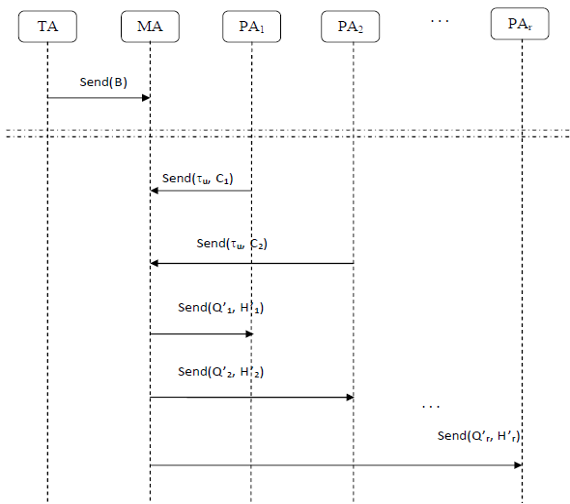
\includegraphics[height=8cm, keepaspectratio]{images/sequence-diagram-case2}
    \caption{Sequence diagram, case 2 – new scheduling, according to the hybrid voting scheme (B = batch file; $Q_i$= work queue; $H_i$= hashes of tasks; $\tau_u$= underloading parameter; C2= cost for the printer 2; $Q\prime_i$= new work queue ; $H\prime_i$= new hashes of tasks)}
    \label{fig:seq-diag-case2}
\end{figure}

\begin{figure}[h]
    \centering
    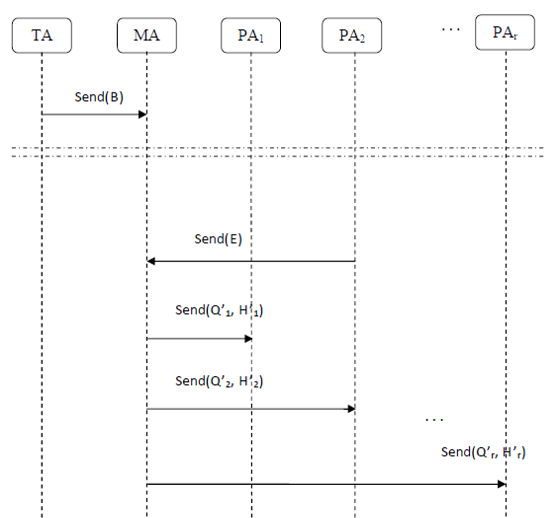
\includegraphics[height=8cm, keepaspectratio]{images/sequence-diagram-case3}
    \caption{Sequence diagram, case 3 – Hash check failed on PA2 (B = batch file; $Q_i$= work queue ; $H_i$= hashes of tasks; $\tau_u$= underloading parameter; C2= new cost for the printer 2; $Q\prime_i$= new work queue ; $H\prime_i$= new hashes of tasks; E=flag for failed check)}
    \label{fig:seq-diag-case3}
\end{figure}

Further work was conducted to outline a basic prototype of a Multi-Agent System for the Cloud Manufacturing network. A modular framework for building, analyzing, and visualizing agent-based models called MESA that uses the Python language has been selected \parencite{masad2015mesa}. More details about the implementation are in Appendix B: A MAS prototype of the CMfg platform.

\section{An implementation of a Scattered Manufacturing Framework for large additive manufacturing networks}
\subsection{Introduction}
In this section, an implementation of a Scattered Manufacturing network for large additive manufacturing scenario is presented. In the proposed scenario, the Scattered Manufacturing Network is constituted of Advanced Manufacturing Technologies nodes that can request or provide production resources (slots) coordinated by an orchestrator, responsible for the communication along with the network, the negotiation among nodes, and the overall (production and logistics) optimization along with the supply chain structure.\\

In this scenario, nodes are either “productive” or “demanding”. Productive nodes provide finished pieces realized by 3D printings. Demanding nodes, instead, orders finished pieces from the productive nodes. In this sense, demanding nodes formulate work orders that are satisfied by the productive ones. Considering complex dynamics inside large networks, one node can often be either productive or demanding in different times or situations. This context suggests that the communication and negotiation activities among nodes, managed by the orchestrator, are fundamental in order to share diverse resources and distribute them along with the network by satisfying principles of transparency and sustainability. In the following paragraphs, dynamics of networks with a unique demanding node and various productive ones are presented. In general, such assumption is not detrimental to the discussion of a general issue, but further details will be described in the last section.
\subsection{Founding Principles}
The network observes three main principles: sustainability, shared resources, and transparency. Sustainability occurs in terms of cost-effective manufacturing, reductions of resource demands, and related CO2 emissions over the entire product life cycle, transferring the production closer to the client. According to the Circular Economy trend, the Scattered Manufacturing Network aims to create a collaborative, transparent, open, and trusting environment with shared purposes and shared resources. In fact, every node in the network can buy resources in the world with an open bidding system, while customers can send demands of products (orders) to the orchestrator. Hence, the orchestrator acts as an intermediate layer collecting orders from many customers.
\subsection{Model description, requirements and network dynamics}
To consider the variables and factors that affect a 3DPs network, a unique model is proposed by combining different approaches, which focus on such needs:
\begin{itemize}
    \item Logistics issues related to the productive nodes that are near the demanding ones.
    \item Possibility of the division of demanding node’s order into subparts and consequent assignment of each subpart to a productive node.
    \item Negotiation criteria between the demanding node and the productive ones in order to establish tradeoffs between different margin strategies.
\end{itemize}

Hence, the orchestrator has a primary role as it behaves like a control unit that applies a multilevel optimization that deals with the following exigencies:
\begin{itemize}
    \item Localization: starting from the demanding node’s geographical position, the orchestrator provides some neighboring nodes that define a “certified” sub-network to satisfy the users’ requests.
    \item Fragmentation and assignment: the orchestrator establishes how to divide the work order into subparts, each assigned to different productive nodes to achieve the lowest overall purchase cost. Notice that this phenomenon requires a suitable negotiation between the demanding node, which asks for a predefined number of pieces, and the productive nodes, that have their quantities and pricing plans.
    \item Picking: the orchestrator defines a closed path that starts from the demanding node and returns to it, touching all the productive nodes once. Such a path, useful to collect the number of pieces from all the productive nodes, is obtained via an approach (see \textcite{karp_patching_1979},\textcite{gutin_traveling_2002},\textcite{traveling_salesman_comp_study},\textcite{gutin2006traveling},\textcite{wang_towards_2016}) that minimizes the logistics costs.
\end{itemize}

Based on the just described requirements, the orchestrator set a run of iterations. As for the first one, the orchestrator:

\begin{itemize}
    \item Indicates suitable productive nodes near the demanding one and assigns them the number of pieces to produce by satisfying constraints dealing with quantity/price plans.
    \item Defines a picking path at minimum logistics cost.
    \item Computes the weights that each productive node has inside the
network. Precisely, for each node, the corresponding weight represents a tradeoff among logistics components, possible quantities of produced pieces, as well as reallocation of quantities by excluding the productive node from the network in consideration. Such last operation is necessary to discriminate among different productive nodes that can be far from the demanding one (hence requiring high logistics costs) but in turn useful due to their advantageous quantity/price plans.
\end{itemize}

As for the second iteration, the orchestrator works as follows. First, the productive node, whose weight indicates the highest decrement of the overall logistics and production costs, is excluded from the network. Then, the orchestrator redefines either the picking path or new fragmentations/assignments to the remaining productive nodes. This last phenomenon triggers a consequent negotiation phase between the demanding node and the productive one, and the result is a tradeoff between different profits. Finally, the orchestrator recalculates the new weights of the remaining productive nodes, and the next iteration works as the second one. Iterations continue until the computation of weights indicates that further decrements of costs are not possible, hence reaching an equilibrium state.

\begin{figure}[h]
    \centering
    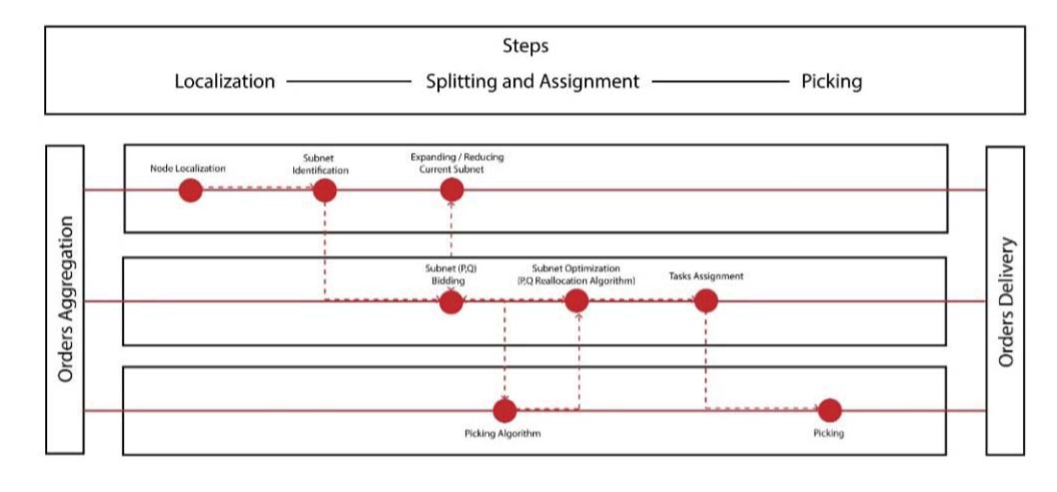
\includegraphics[height=4cm, keepaspectratio]{images/visual-repr-steps-algorithm}
    \caption{A visual representation of the steps involved in the proposed algorithm}
    \label{fig:visual-repr-steps-algorithm}
\end{figure}

Indeed, the originality and the contribution of the proposed approach foresees a complete balance among exigencies of different nodes. Starting from localization requests of the demanding node that needs a certified service network, a unique framework mixes approaches for picking paths and resource allocation problems that solve issues of fragmentation and assignment. Such aspects are dependent on each other, as they are strictly connected by the weights that the various productive nodes have inside the network. Indeed, the possible exclusion of productive nodes from the network determines a guideline to solve at the same time logistics issues, as well as reallocations by considering the overall quantity/price plans of each productive node. This last aspect, which clearly deals with the negotiation phases between the demanding node and the productive ones, represents the effective dynamics of the network at each iteration provided by the orchestrator.\\
The next paragraphs present a mathematical model followed by numerical examples. These examples show either expected features or unexpected ones. For instance, it is possible that the exclusion of a node during the iterations could provoke increments of logistics costs, as well as a suitable reduction of productive purchase. This situation implies the consequent need for new iterations. The tradeoff between logistics and production components indicates that the nodes to exclude do not obey a predefined and precise rule. Moreover, networks of medium dimensions might reach an equilibrium state in just one iteration. Such a phenomenon is important as it indicates that larger networks are sometimes easier to manage.

\subsection{Modeling a 3DPs network}
This paragraph briefly describes some features for a Scattered Manufacturing network within the context of 3DPs. The Scattered Manufacturing network is composed by a set of nodes $V = \left\{v_1,v_2,...,v_n \right\}$  while the network is characterized by:
\begin{itemize}
    \item $e_{ij}$ is the arc that connects nodes $v_i$ and $v_j$;
    \item $c_{ij}$ is the cost for arc $e_ij$;
\end{itemize}

Notice that $c_{ij}$ depends on various factors, such as the distance between  $v_i$ and $v_j$, the overall monetary cost for transports, the traveling time, as well as criteria of sustainability. Parameters  are kept in a coefficient matrix:

\begin{equation}
    \label{eq:11}
    X = \begin{pmatrix}c_{ij}\end{pmatrix}_{i,j=1,...,N}
\end{equation}

The SM network is assumed to be bidirectional, namely: two different nodes $v_i$ and $v_j$ are connected in the direction either “from $v_i$ to $v_j$ ” or “from $v_j$ to $v_i$”. Obviously, $e_{ij}$ - and $e_{ji}$ - are the same arc while, in general, $c_{ij} \neq c_{ji}$.
Each node provides services to the users in terms of finished pieces produced by 3DPs. Quantities $Q_i$ and prices $P_i$ of pieces for a generic node $v_i$ obey a “law at three levels” of type:

\begin{equation}
    \label{eq:12}
    P_i(Q_i) = 
    \begin{cases} 
        p^i_L & if  0 < Q_i \leq k^i_L \\
        p^i_M & if  k^i_L  < Q_i \leq k^i_M \\
        p^i_H & if  k^i_M  < Q_i \leq k^i_H \\
    \end{cases}
\end{equation}
with $p^i_L<p^i_M,p^i_H$. The interpretation is the following: if the required quantity $Q_i$ does not exceed $k^i_L$, the price $P_i$ is the lowest $p^i_L$; otherwise, possible prices are $p^i_M$ and $p^i_H$.\\
Notice that \ref{eq:12} represents a possible and realistic attempt to describer the evolution of pieces versus their possible prices. Indeed, future research activities aim at guaranteeing more suitable shapes for \ref{eq:12}, with the aim of describing negotiation criteria among nodes.

\subsection{Modeling a demanding node}

This paragraph shortly describes a possible approach for optimizing demanding node’s needs inside a 3DPs network. In particular, a unique model is described in which more approaches, often used individually, are used.\\
The demanding node aims to obtain a series of services from the Scattered Manufacturing network. In the specific case, in a preliminary phase, the orchestrator helps the demanding node referring to the following issues:
\begin{itemize}
    \item \textit{Localization}: the orchestrator makes the demanding node become the center of a circle with a radius of “economic” type. This means that, according to the demanding node’s geographical position, only some production nodes belonging to an area tracked by the orchestrator are able to offer services. Such a localization criterion has the advantage of defining the most known and neighboring nodes, thus creating a sort of “certified” sub-network. Therefore, the demanding node might have a higher level of trust. Each available node of the certified sub-network shows its offer in terms of prices/quantities plans.
    \item \textit{Fragmentation and Assignment}: the orchestrator, considering the features of the sub-network, decides how to fragment the demanding node’s work order and how to assign the various subparts to the production nodes in order to get the lowest purchase costs.
    \item \textit{Picking}: the orchestrator chooses a closed path, which starts and returns to the demanding node through all the production nodes once. The path is defined via an approach described by the procedure shown as follows (see for details \textcite{karp_patching_1979},\textcite{gutin_traveling_2002},\textcite{traveling_salesman_comp_study},\textcite{gutin2006traveling},\textcite{wang_towards_2016}).
\end{itemize}

\subsection{The picking algorithm}
For a Scattered Manufacturing network whose features are described in previous paragraphs, the following procedure is used for the picking activities. Assume that $P$ is a possible closed path that crosses each node of $V$, starting from a source node $ v_s \in V$ and coming back to it; $C(P)$ is the cost associated to $P$.
\begin{algorithm}
    \caption{Picking algorithm (PA)}
    \label{listing7}
    \begin{algorithmic}[1]
        \Procedure{Initialization}{}
        \State $P : = \emptyset, C(P) : = \emptyset, v_s : = v_j \in V$.
        \EndProcedure
        \Procedure{Steps}{}
        \State 1. From node $v_j$ go to node $v_i \in V\setminus\{v_j\}$ such that $c_{ji} = \min\cup^{|V|}_{i=1,i\neq j} c_{ji}$
        \State 2. $P \leftarrow P \cup e_{ji}, C(P) \leftarrow C(P)P + c_{ji}, V \leftarrow V\setminus \{v_j\}$ 
        \State 3. \If If $|V| = 1, P \leftarrow P\cup e_{ij}$ \Return end of the algorithm; \Else  $v_j \leftarrow v_I$ and go to step 1 \EndIf
        \EndProcedure
    \end{algorithmic} 
\end{algorithm}

Considering a SM network with $V = \{v1, v2, v3, v4\}$ and matrix $X$:
\begin{equation}
    \label{eq:x-matrix-sample-initialization}
    X = \begin{pmatrix} 0 & 5 & 9 & 1\\ 3 & 0 & 7 & 11\\ 7 & 9 & 0 & 8\\ 2 & 12 & 6 & 0 \end{pmatrix}
\end{equation}

Preliminary, $P : = \emptyset , C(P) : = 0, v_s : = v_1$. Table \ref{tab:evolution-of-iterations} shows the various iterations. Figure 19, where numbers indicate the nodes for simplicity, presents a graphical evolution of the path.
\begin{table}
    \centering
    \begin{tabular}{|c|c|c|c|}
        \hline
        \textbf{Iteration} & \textbf{P} & \textbf{C(P)} & \textbf{V} \\
        \hline
        1 & $\{e_{14}\}$ & 1 & $\{2,3,4\}$\\
        \hline
        2 & $\{e_{14}, e_{43}\}$ & 7 & $\{2,3\}$\\
        \hline
        3 & $\{e_{14}, e_{43}, e_{32}\}$ & 16 & $\{2\}$\\
        \hline
        4 & $\{e_{14}, e_{43}, e_{32}, e_{21}\}$ & 19 & $\{2\}$\\
        \hline
    \end{tabular}

    \caption{Evolution of the iterations}
    \label{tab:evolution-of-iterations}
\end{table}


\begin{figure}[h]
    \centering
    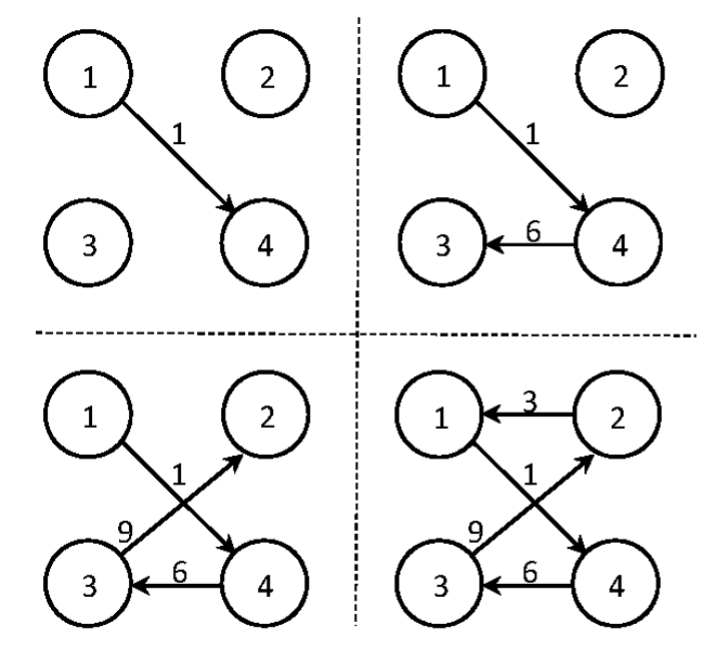
\includegraphics[height=8cm, keepaspectratio]{images/graphical-evolution-of-path}
    \caption{Graphical Evolution of the path}
    \label{fig:graphical-evolution-of-path}
    \small{\textit{Iteration 1 (up, left): the first arc of the path $P$ connects nodes $v_1$ and $v_4$. Iteration 2 (up, right): the path $P$ connects nodes $v_4$ and $v_3$. Iteration 3 (bottom, left): the path $P$ connects nodes $v3$ and $v2$. Iteration 4 (bottom, right): the path $P$ connects nodes $v_2$ and $v_1$.}}
\end{figure}

\subsection{Combining issues of Localization, Fragmentation, Assignment and Picking}
Considering a demanding node that asks for services from a generic Scattered Manufacturing network, the aim is to decrease the overall cost. The cost function has two components, $C_X$ and $C_Y$, that refer to the logistics (associated with the path) and the manufacturing costs, respectively. A suitable algorithm that considers all exigencies of the demanding role is presented in what follows.\\
Consider a preliminary phase (iteration 0). The orchestrator, referring to a Scattered Manufacturing network with M nodes (Figure 20, up left), tracks an economic radius for the demanding node (in position $T$ in Figure 20, upright), discriminates the unreliable nodes (in red, Figure 20, bottom left), defines a closed path $P$ from $T$ to $T$ according to algorithm (PA), and computes the weights of each production node inside the network.\\
Notice that $P$ has production nodes for which, respecting constraints of fragmentation and assignment, purchase costs occur. Hence, at the iteration 0, $C_X$ and $C_Y$ are as follows: $C^{(0)}_X = C(P)$ and $C^{(0)}_Y=\sum^{N}_{i=1}p^i_L$.
\begin{figure}[h]
    \centering
    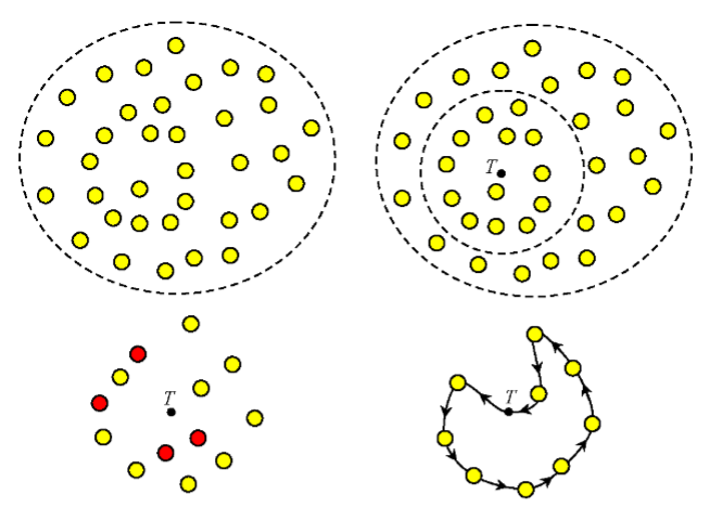
\includegraphics[height=8cm, keepaspectratio]{images/prelim-phase-it0}
    \caption{Preliminary phase (iteration 0)}
    \label{fig:prelim-phase-it0}
\end{figure}
For further iterations, the orchestrator works as follows in order to decrease the overall costs:
\begin{itemize}
    \item Deleting nodes that can provoke the lowest costs in the next iteration.
    \item Reallocation of the sub-parts of the work orders (a new fragmentation and assignment phase), with consequent negotiation between the demanding node and the productive nodes. Notice that reallocation activities foresee a possible saturation of productive nodes.
    \item Computation of a new path for picking by using Listing 7: Picking algorithm (PA).
    \item Calculation of new weights (reallocation parameters) associated with the productive nodes.
\end{itemize}
Notice that removing nodes from the network implies an obvious natural variation of either logistic or purchase costs. In order to understand the entity of variations and compute the weights for the productive nodes, we define the following quantities:
\begin{itemize}
    \item $\Delta C^{v_i}_X$, that represent the variation of the logistics costs when a node $v_i$ is excluded from the network. Precisely, we have that $\Delta C^{v_i}_X = C(P) - C(P\setminus v_i)$.
    \item $\Delta C^{v_i}_Y$ that indicates the dynamics of purchase costs when a node $v_i$ is excluded from the network. In detail, we get that: $\Delta C^{v_i}_Y = -Q_i \left[P_i (Q_i)\right] + \sum^{|V|}_{j=1,i \neq j} Q\prime _j P_j (Qj + Q\prime _j)$, where $P_i (Q_i)$ follows \ref{listing7} while $Q\prime _j$ is the amount of pieces redistributed on the network using the reallocation algorithm (RA), described above.
    \item $\Delta R^{v_i} = \Delta C_X^{v_i} + \Delta C_Y^{v_i}$ is the weight (reallocation parameter) associated to node $v_i$. Notice that, if $\Delta R^{v_i} < 0$, the exclusion of node $v_i$ allows a decrement in the overall cost for the network.
\end{itemize}

\subsection{Reallocation algorithm (RA)}
Assume that $L$ is the total amount of pieces, which the demanding nodes require from the network.\\
If node $v_i$ is excluded from the network, $Q_i$ is redistributed among nodes. The new quantity $Q\prime _j , j=1, ..., |V|, j \neq i$, is defined as follows:
\begin{equation}
    \label{eq:RA-new-quantities}
    Q\prime _j = \left\lceil \frac{Q_i}{|V| - 1} \right\rceil
\end{equation}
such that:
\begin{equation}
    \label{eq:RA-lot-parity}
    \sum^{|V|}_{j=1,j \neq i} Q\prime _j = L
\end{equation}
Notice that Equation \ref{eq:RA-new-quantities} has the following interpretation: as the productive nodes have all the same importance for the demanding node, the quantity $Q_i$ is equally distributed among all the other remaining productive nodes. If $\frac{Q_i}{|V| - 1}$ is not integer, then the whole upper part is taken.\\
Finally, the overall optimization algorithm, defined by the orchestrator’s activities, works as follows, at the n-th iteration:
\begin{itemize}
    \item Step 1: Erase the node $j_n$ whose weights allows a reduction of the overall costs for the network in consideration. 
    \item Step 2: Compute a new path for picking, with new cost $C_X^{(n)}$
    \item Step 3: Reallocate the quantities of pieces $Q_i , i=1, i \neq j$ of each node according to the reallocation algorithm (RA).
    \item Step 4: Compute the new weights for productive nodes.
    \item Step 5: Come back to step 1 if there is at least one reallocation parameter $\Delta R^{v_i}$ is negative.
\end{itemize}
Figure 21 provides an intuitive idea of the optimization algorithm, considering the second, the third and then the n-th iteration.

\begin{figure}[h]
    \centering
    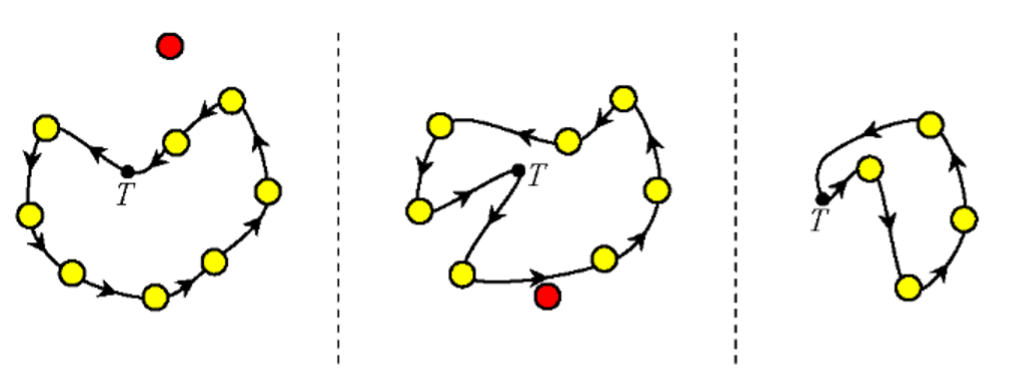
\includegraphics[height=4cm, keepaspectratio]{images/viz-repr-optim-alg}
    \caption{A visual representation of the optimization algorithm}
    \label{fig:viz-repr-optim-alg}
    \small{\textit{Left: in the second iteration, a node (in red) is excluded, the picking path is recomputed, the logistics cost decreases while the overall purchase one can remain the same or decrease. Center: in the third iteration, another node is excluded, and the process continues. Right: in the n-th iteration, the overall logistics and purchase costs are highly decreased}}
\end{figure}

\subsection{Numerical examples of the proposed algorithm}
The following example shows the numerous algorithm steps.
\subsubsection{Example A}
Consider a Scattered Manufacturing network with $V = \{v_1,v_2,v_3,v_4, v_5, v_6\}$ and matrix $X = \begin{pmatrix} c_{ij} \end{pmatrix} _{i,j=1,...,6}$. A possible interpretation of the starting phase (iteration 0) is in Figure 22. The preliminary closed path $P$ (Figure 22, up) involves the demanding node, $v_i$, and the productive nodes $v_2, v_3, v_4, v_5$ and $v_6$. For the productive nodes, the orchestrator determines purchase costs of $p_L$ type (Figure 22, down), together with suitable assignments of finished pieces, as well as weights of each productive node inside the network.

\begin{figure}[h]
    \centering
    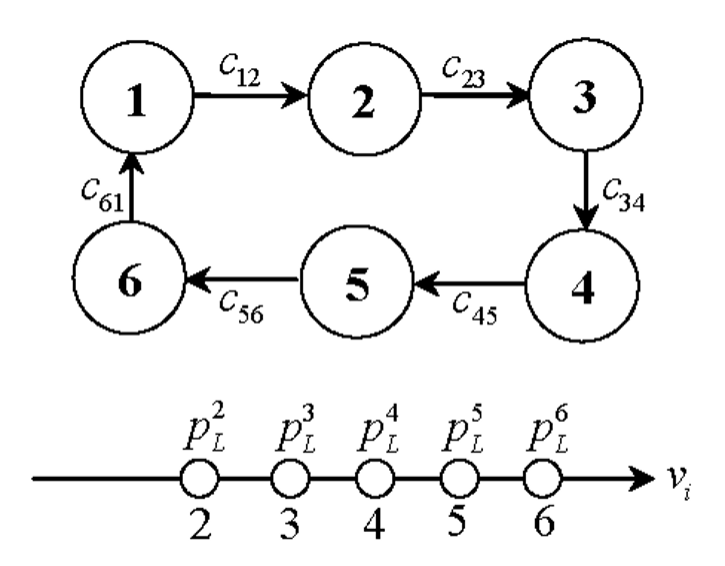
\includegraphics[height=4cm, keepaspectratio]{images/exempleA-it0}
    \caption{Example A, iteration 0}
    \label{fig:exempleA-it0}
\end{figure}
At iteration 1:
\begin{itemize}
    \item Node $v_3$ is excluded because it has the lowest reallocation parameter.
    \item The closed path $P$ is recomputed using algorithm (PA) considering the set $V = \{v_1,v_2,v_3,v_4, v_5, v_6\}$. 
    \item A cost $C^{(1)}_X$ is obtained
    \item A new fragmentation/assignment is made for the nodes of set $V$, see reallocation algorithm (RA).
    \item A cost $C^{(1)}_Y$ is obtained.
    \item New weights for productive nodes are computed.
\end{itemize}
Figure \ref{fig:exempleA-it1} sums up the iteration 1.

\begin{figure}[h]
    \centering
    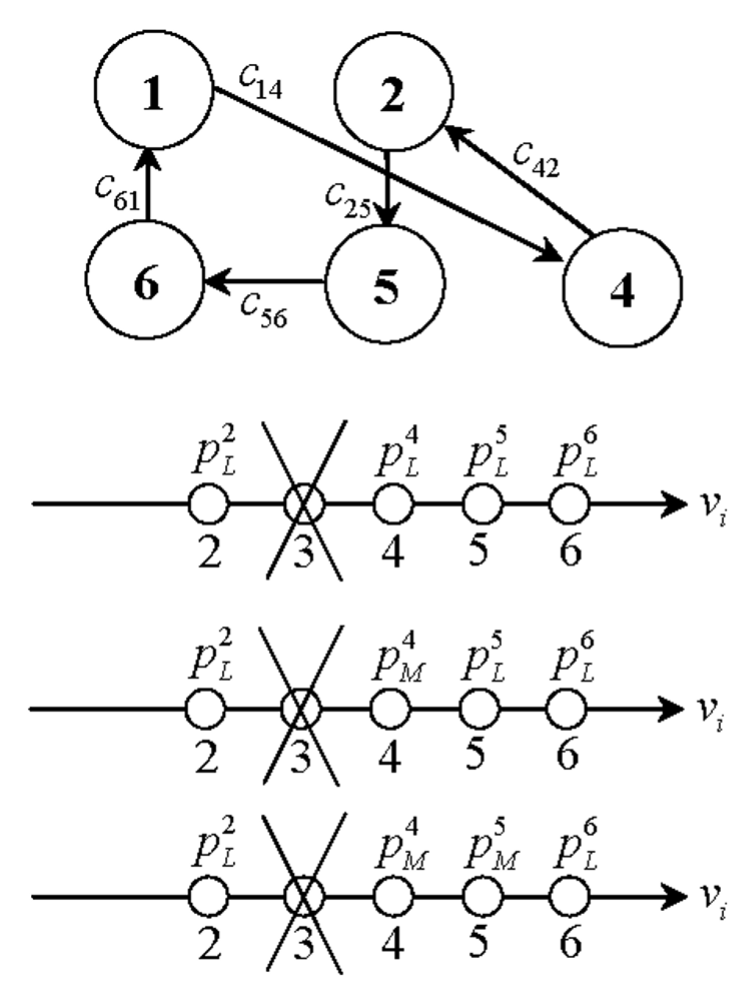
\includegraphics[height=8cm, keepaspectratio]{images/exempleA-it1}
    \caption{Example A, iteration 1}
    \label{fig:exempleA-it1}
\end{figure}
Precisely, Figure \ref{fig:exempleA-it1} (up) presents the new path, while Figure \ref{fig:exempleA-it1} (bottom) shows possible scenarios for $C^{(1)}_Y$:
\begin{itemize}
    \item Scenario 1.1 (no variations): $p^3_L$ is erased and all other prices of $p_L$ type remain the same.
    \item Scenario 1.2 (variations of just one cost): $p^3_L$ is erased, $p^4_L$ becomes $p^4_M$ and all other prices of $p_L$ type remain the same.
    \item Scenario 1.3 (variations of more costs): $p^3_L$  is erased while, for instance, $p^4_L$ and $p^5_L$ become, respectively, $p^4_M$ and $p^5_M$.
\end{itemize}

Assuming that the scenario 1.2 occurs, at the iteration 2:
\begin{itemize}
    \item Node $v_2$ is excluded due to its weight.
    \item The closed path $P$ is obtained via algorithm (PA) for the new set $V = \{v_1,v_2,v_3,v_4, v_5, v_6\}$.
    \item A cost $C_X^{(2)}$ is computed.
    \item A new fragmentation/assignment occurs for the nodes of $V$ see reallocation algorithm (RA).
    \item A cost $C^{(2)}_Y$ is computed.
    \item New weights for productive nodes are established.
\end{itemize}

Figure \ref{fig:exempleA-it2} presents the iteration 2.
\begin{figure}[h]
    \centering
    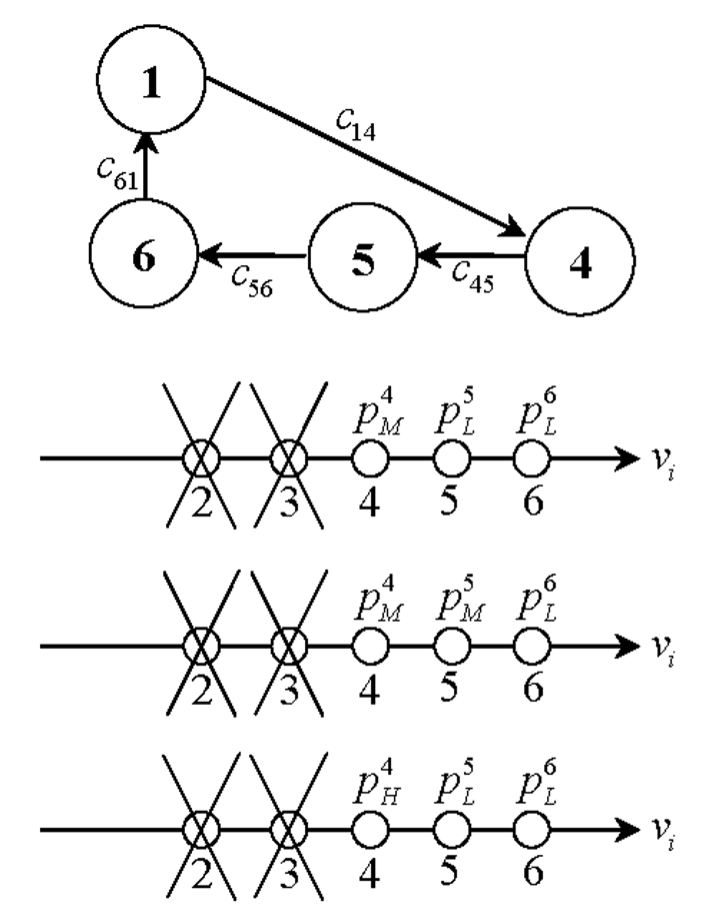
\includegraphics[height=8cm, keepaspectratio]{images/expA-it2}
    \caption{Example A, iteration 2}
    \label{fig:exempleA-it2}
\end{figure}
Precisely, Figure \ref{fig:exempleA-it2} (up) considers the new path, while Figure \ref{fig:exempleA-it2}  (bottom) indicates possible new scenarios for $C_Y^{(2)}$:
\begin{itemize}
    \item Scenario 2.1 (no variations): $p_L^2$ is erased while all other nodes have prices foreseen in scenario 1.2.
    \item Scenario 2.2 (variations of just one cost): $p_L^2$ is erased, $p_L^5$ becomes $p_M^5$ while all other nodes have prices described in the scenario 1.2.
    \item Scenario 2.3 (a high cost is achieved): $p_L^2$ is erased, $p_M^4$ becomes $p_H^4$ while all other nodes have prices described in scenario 1.2. In this case, the algorithm ends, as one term of $p_H$ type is obtained, and all reallocation parameters become positive.
\end{itemize}
Assuming that the scenario 2.2 occurs, at the iteration 3:
\begin{itemize}
    \item Node $v_6$ is excluded;
    \item A new closed path $P$ is computed by picking algorithm (PA) for the new set $V = \{v_1, v_4, v_5\}$;
    \item A cost $C^{(3)}_X$ is obtained;
    \item A new fragmentation/assignment is made for the nodes of $V$, see reallocation algorithm (RA);
    \item A cost $C_Y^{(3)}$ is considered;
    \item Weights for productive nodes are updated.
\end{itemize}
Figure \ref{fig:expA-it3} presents the iteration 3.
\begin{figure}[h]
    \centering
    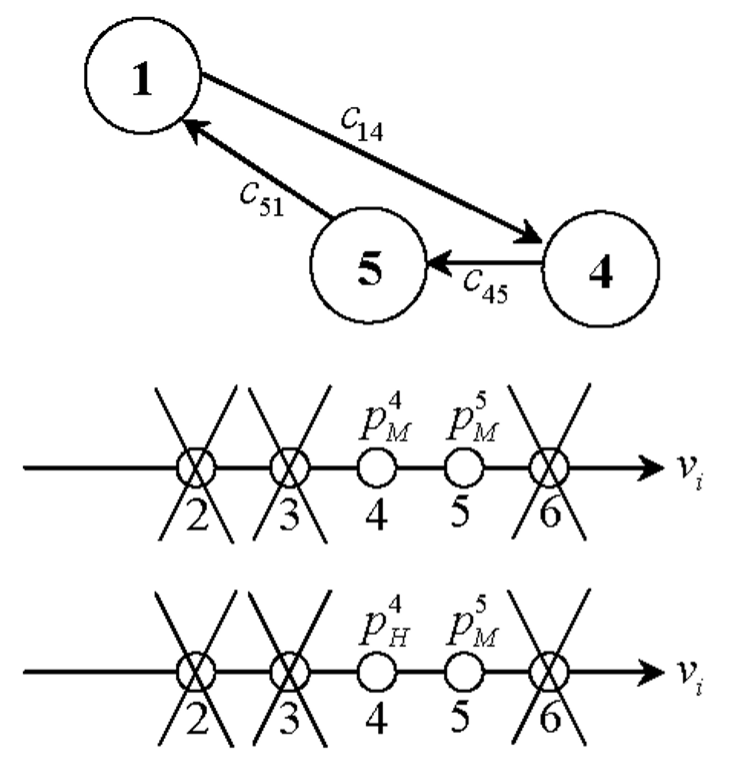
\includegraphics[height=6cm, keepaspectratio]{images/expA-it3}
    \caption{Example A, iteration 3}
    \label{fig:expA-it3}
\end{figure}

In particular, Figure \ref{fig:expA-it3} (up) shows the new path, while Figure \ref{fig:expA-it3} (bottom) presents possible various scenarios for $C_Y^{(3)}$:
\begin{itemize}
    \item Scenario 3.1 (no variations): $p_L^6$ is erased while all other nodes have prices foreseen in the scenario 2.2.
    \item Scenario 3.2 (variations of just one cost): $p_L^6$ is erased, $p_M^4$ becomes $p_H^4$ while all other nodes have prices described in scenario 2.2. The algorithm ends, as one term of $p_H$ type is obtained, and all reallocation parameters become positive.
\end{itemize}

\subsection{Numerical tests}
This paragraph is devoted to some numerical tests. In particular, each of them presents some features that are useful to provide a better idea of dynamics inside a Scattered Manufacturing network.
\paragraph{Test 1}
Starting with a Scattered Manufacturing network with $V = \left\{v_1, v_2, v_3, v_4 \right\}$ set of nodes and a matrix $X$: $$X = \begin{pmatrix}\infty & 10 & 40& 30\\ 10 & \infty & 20 & 50 \\ 40 & 20 & \infty & 40\\ 30 & 50 & 40 & \infty \end{pmatrix}$$
Assume that $P : = \emptyset, C(P) : = 0, v_s : = v_1$. Hence, the demanding nodes is $v_1$ while node $v_j, j = 2, 3, 4$ is of productive type. Price/quantity plans follow the formulation \ref{eq:12} with $p_L^2 = 25, p_L^3 = 20, p_L^4 = 15, p_M^2 = 30, p_M^3 = p_M^4 = 25; p_H^2=35, p_H^3= p_H^4 = 45; k_l^2=40, k_L^3 =50, k_L^4 = 70; k_M^2 = 50, k_M^3 = 90, k_M^4 = 95; k_H^2=60, k_M^3 = k_M^4 =95$.\\
The total amount of pieces requested is $L = 100$ among the productive nodes $v_2, v_3 and v_4$. Preliminarily, the orchestrator indicates $Q_2 = 10, Q_3 = 30 and Q_4 = 50$. Such quantities are offered at prices $p_L^2, p_L^3$ and $p_L^4,$, respectively.
The iterations run as follows.
\textit{First iteration:}
From algorithm (PA), we have $P : = 100 = C_X^{(1)}$. As $Q_2^{(1)} = Q_2 = 10, Q_3^{(1)} = Q_3 = 30$ and $Q_4^{(1)} = Q_4 = 50$ ,from the preliminary fragmentation we get $C_Y^{(1)} = Q_2^{(1)} p_L^2 + Q_3^{(1)} p_L^3 + Q_4^{(1)} p_L^4$. Therefore, $ C_{TOT}^{(1)} = 1700$.\\
By considering the computation of weights for nodes, as well as the reallocation via algorithm (RA), Table \ref{tab:dyn-logistics-path-first-it} is obtained.

\begin{table}
    \centering
    \begin{tabular}{|c|c|c|c|c|}
        \hline
        \textbf{Nodes} & \textbf{$P \setminus v_i$} & \textbf{$\Delta C_X^{v_i}$} & \textbf{$\Delta C_Y^{v_i}$} & \textbf{$\Delta R^{v_i}$} \\
        \hline
        $v_2$ & $\left\{e_14, e_43, e_31 \right\}$ & +10 & -75 & -65 \\
        \hline
        $v_3$ & $\left\{e_12, e_24, e_41 \right\}$ & -10 & 0 & -10 \\
        \hline
        $v_4$ & $\left\{e_12, e_23, e_31 \right\}$ & -30 & +375 & -345 \\
        \hline
    \end{tabular}

    \caption{Dynamics of logistics paths, costs and reallocations for the first iteration}
    \label{tab:dyn-logistics-path-first-it}
\end{table}

From Table \ref{tab:dyn-logistics-path-first-it}, node 2 must be excluded in the next iteration.\\
\textit{Second iteration:}
We get $P : = \left\{e_{14}, e_{43}, e_{31}\right\}, C : = 110 = C_X^{(2)}$. Moreover, $Q_3^{(2)} = 35$ and $Q_4^{(2)} = 55$ at prices $p_L^3$ and $p_L^4$ and $C_Y^{(2)} = Q_3^{(2)} p_L^3 + Q_4^{(2)} p_L^4 = 1525$. Hence, $C_{TOT}^{(2)} = 1635$. Table \ref{tab:reallocation-plan-second-it} shows the posisble reallocations and variations of costs for the next iteration.

\begin{table}
    \centering
    \begin{tabular}{|c|c|c|c|c|}
        \hline
        \textbf{Nodes} & \textbf{$P \setminus v_i$} & \textbf{$\Delta C_X^{v_i}$} & \textbf{$\Delta C_Y^{v_i}$} & \textbf{$\Delta R^{v_i}$} \\
        \hline
        $v_3$ & $\left\{e_{14}, e_{41}, \right\}$ & -50 & +725 & +675 \\
        \hline
        $v_4$ & $\left\{e_{13}, e_{31} \right\}$ & -30 & +275 & +245 \\
        \hline
    \end{tabular}

    \caption{Reallocation plan for the second iteration}
    \label{tab:reallocation-plan-second-it}
\end{table}

As Table \ref{tab:reallocation-plan-second-it} indicates that $\Delta R_{v_i} > 0, i = 3,4$, the possible exclusion of nodes $v_3$ and $v_4$ does not imply a reduction of the overall cost. Hence, the iterations stop. From the following example, we consider two important phenomena. First, the exclusion of a node from the network does not necessarily imply a reduction of the logistics costs. This is due to the recalculation of the new picking path, which can be very different, also in terms of costs associated to arcs, from the ones of the previous iterations. Second, for the last iteration node $v_2$ is not considered. At a first sight, one expects that this could occur for node $v_4$ as $\Delta C_X^{v_4} < \Delta C_X^{v_2}$. Indeed, as $\Delta C_Y^{v_4} >> \Delta C_Y^{v_2}$ the possible exclusion of node $v_4$. implies the worst case for the overall cost, that increases considerably. Hence, although node $v_2$, unlike $v_4$, is the less advantageous in logistics terms for the demanding node $v_1$, it should be avoided due to an higher fluctuations of the production cost.\\
\paragraph{Test 2}
Consider a SM network with $V = \left\{v_1, v_2, v_3, v_4, v_5, v_6, v_7 \right\}$ and a matrix $X$: $$X = \begin{pmatrix}\infty & 10 & 25 & 5 & 7 & 9 & 13\\ 14 & \infty & 171 & 21 & 12 & 5 & 12 \\ 11 & 15 & \infty & 14 & 13 & 12 & 14\\ 11 & 10 & 9 & \infty & 17 & 12 & 13 \\ 15 & 12 & 11 & 9 & \infty & 14 & 18\\ 12 & 13 & 17 & 17 & 19 & \infty & 15\\ 13 & 11 & 9 & 13 & 15 & 17 & \infty \end{pmatrix}$$
The demanding node is represented by $v_i$ while node $v_j , j=2, ..., 7$, is of productive type. For productive nodes, prince/quantity functions have levels shown in Table \ref{tab:network-price-quantity-plans}.

\begin{table}[h]
    \centering
    \begin{tabular}{|c|c|c|c|c|c|c|}
        \hline
        \textbf{Nodes} & \textbf{$p_L^i$} & \textbf{$p_M^i$} & \textbf{$p_H^i$} & \textbf{$k_L^i$} & \textbf{$k_M^i$} & \textbf{$k_H^i$} \\
        \hline
        $v_2$ & 25 & 35 & 45 & 15 & 25 & 35\\
        \hline
        $v_3$ & 35 & 45 & 55 & 20 & 40 & 50\\
        \hline
        $v_4$ & 30 & 40 & 60 & 25 & 35 & 50\\
        \hline
        $v_5$ & 20 & 30 & 45 & 10 & 25 & 40\\
        \hline
        $v_6$ & 30 & 45 & 60 & 15 & 25 & 35\\
        \hline
        $v_7$ & 30 & 40 & 50 & 25 & 40 & 55\\
        \hline
    \end{tabular}

    \caption{Network price/quantity plans}
    \label{tab:network-price-quantity-plans}
\end{table}

Assume that $P : = \emptyset, C(P) : = 0, v_s : = v_1$. In this case, $L = 80$ pieces that should be scheduled among the productive nodes. At the beginning of the current iteration, the orchestrator provides $Q_2 = 10, Q_3 = 15, Q_4 = 20, Q_5 = 5, Q_6 = 10, Q_7 = 20$, at prices $p_L^i , i=2,...,7$. The iterations run as follows.\\
\textit{First iteration:}\\
Picking algorithm (PA), we have $P : = \left\{e_{14},e_{43}, e_{36}, e_{62}, e_{25}, e_{57}, e_{71}\right\}$, $C(P) : = 82 = C_X^{(1)}$. As $Q_i^{(1)} = Q_i, i=2,...,7$ and the result $C_Y^{(1)} = \sum^{7}_{i=2} Q_i^{1} p_L^i = 2375$, and $C_{TOT}^{(1)} = 2457$.\\
Computing the weights for nodes involved and applying the reallocation algorithm (RA), Table \ref{tab:reallocation-plan-second-it} is obtained.

\begin{table}
    \centering
    \begin{tabular}{|c|c|c|c|c|}
        \hline
        \textbf{Nodes} & \textbf{$P \setminus v_i$} & \textbf{$\Delta C_X^{v_i}$} & \textbf{$\Delta C_Y^{v_i}$} & \textbf{$\Delta R^{v_i}$} \\
        \hline
        $v_2$ & $\left\{e_{14}, e_{43}, e_{36}, e_{67}, e_{75}, e_{51} \right\}$ & -11 & +40 & +29 \\
        \hline
        $v_3$ & $\left\{e_{14}, e_{42}, e_{26}, e_{67}, e_{75}, e_{51} \right\}$ & -17 & -120 & -137 \\
        \hline
        $v_4$ & $\left\{e_{15}, e_{53}, e_{36}, e_{62}, e_{27}, e_{71} \right\}$ & -14 & +100 & +86 \\
        \hline
        $v_5$ & $\left\{e_{14}, e_{43}, e_{36}, e_{62}, e_{27}, e_{71} \right\}$ & -18 & +50 & +32 \\
        \hline
        $v_6$ & $\left\{e_{14}, e_{43}, e_{35}, e_{52}, e_{27}, e_{71} \right\}$ & -18 & +50 & +32 \\
        \hline
        $v_7$ & $\left\{e_{14}, e_{43}, e_{36}, e_{62}, e_{25}, e_{51} \right\}$ & -16 & +50 & +34 \\
        \hline
    \end{tabular}

    \caption{Possible logistics paths, costs and reallocations for the first iteration}
    \label{tab:reallocation-plan-second-it}
\end{table}

Table \ref{tab:reallocation-plan-second-it} foresees that node $v_3$ must not be considered in the second iteration.\\
\textit{Second iteration:}\\
In this case, the new path is $P : = \left\{e_{14},e_{42}, e_{26}, e_{67}, e_{75}, e_{51} \right\}$, $C(P) : = 65 = C_X^{(2)}$. We get that $Q_2^{(2)} = 13, Q_4^{(2)} = 24, Q_5^{(2)} = 8, Q_6^{(2)} = 13, Q_7^{(2)} = 23, $ while $C_Y^{(2)} = 2255$, and $C_{TOT}^{(2)} = 2320$.\\
As for the computation of reallocation parameters, we refer to Table \ref{tab:second-test-reallocation-second-iteration}.

\begin{table}
    \centering
    \begin{tabular}{|c|c|c|c|c|}
        \hline
        \textbf{Nodes} & \textbf{$P \setminus v_i$} & \textbf{$\Delta C_X^{v_i}$} & \textbf{$\Delta C_Y^{v_i}$} & \textbf{$\Delta R^{v_i}$} \\
        \hline
        $v_2$ & $\left\{e_{14}, e_{46}, e_{67}, e_{75}, e_{51} \right\}$ & -3 & +905 & +902 \\
        \hline
        $v_4$ & $\left\{e_{15}, e_{52}, e_{26}, e_{67}, e_{71} \right\}$ & -13 & +800 & +787 \\
        \hline
        $v_5$ & $\left\{e_{14}, e_{42}, e_{26}, e_{67}, e_{71} \right\}$ & -17 & +70 & +53 \\
        \hline
        $v_6$ & $\left\{e_{14}, e_{42}, e_{25}, e_{57}, e_{71} \right\}$ & -7 & +925 & +918 \\
        \hline
        $v_7$ & $\left\{e_{14}, e_{42}, e_{26}, e_{65}, e_{51} \right\}$ & -11 & +1010 & +999 \\
        \hline
    \end{tabular}

    \caption{Parameters variation for the second iteration}
    \label{tab:second-test-reallocation-second-iteration}
\end{table}

The iteration stops because $\Delta R^{v_i} > 0 , i = 2,4,5,6,7$. Moreover, the higher increments of terms $\Delta C_Y^{v_i}, i = 2,4,5,6,7$, are essentially due to the fact that prices become of type $p_M$. Such an event, indeed, does not always indicate very high discrepancies, as shown by $\Delta C_Y^{v_5}$.\\
Notice that the described example presents how a network of medium dimensions can reach an equilibrium situation in just one iteration. This suggests that suitable policies of choosing productive nodes could foresee to enlarge the economic radius in order to achieve higher advantages in terms of lower costs.

\paragraph{Test 3}
Scattered Manufacturing network with $V = \left\{ v_{1}, v_{2}, v_{3}, v_{4}, v_{5}, v_{6}, v_{7}, v_{8}, v_{9}, v_{10}, \right\}$ and matrix X: 
$$X = \begin{pmatrix} 
    \infty & 10 & 15 & 17 & 12 & 11 & 17 & 18 & 19 & 22\\
    14 & \infty & 11 & 18 & 17 & 24 & 14 & 22 & 18 & 20\\
    17 & 20 & \infty & 22 & 21 & 22 & 23 & 24 & 18 & 19\\
    17 & 16 & 15 & \infty & 19 & 21 & 24 & 23 & 22 & 21\\
    19 & 21 & 22 & 17 & \infty & 22 & 21 & 20 & 19 & 17\\
    20 & 21 & 22 & 23 & 24 & \infty & 24 & 22 & 21 & 19\\
    18 & 17 & 18 & 15 & 14 & 19 & \infty & 21 & 22 & 24\\
    15 & 18 & 21 & 24 & 27 & 22 & 21 & \infty & 18 & 20\\
    38 & 37 & 35 & 32 & 44 & 42 & 41 & 41 & \infty & 40\\
    15 & 18 & 18 & 17 & 16 & 17 & 18 & 19 & 21 & \infty
\end{pmatrix}$$
Assuming $v_1$ as the demanding node, while node $v_j = 2,...,7$, are the productive ones. Levels of price/quantity plans are in Table \ref{tab:network-price-quantity-plan-test3}
\begin{table}[h]
    \centering
    \begin{tabular}{|c|c|c|c|c|c|c|}
        \hline
        \textbf{Nodes} & \textbf{$p_L^i$} & \textbf{$p_M^i$} & \textbf{$p_H^i$} & \textbf{$k_L^i$} & \textbf{$k_M^i$} & \textbf{$k_H^i$} \\
        \hline
        $v_2$ & 10 & 12 & 15 & 20 & 25 & 35\\
        \hline
        $v_3$ & 15 & 18 & 20 & 25 & 30 & 40\\
        \hline
        $v_4$ & 10 & 11 & 12 & 25 & 35 & 50\\
        \hline
        $v_5$ & 15 & 17 & 19 & 35 & 45 & 50\\
        \hline
        $v_6$ & 25 & 28 & 30 & 35 & 55\\
        \hline
        $v_7$ & 25 & 28 & 30 & 30 & 35 & 55\\
        \hline
        $v_8$ & 15 & 18 & 21 & 15 & 20 & 25\\
        \hline
        $v_9$ & 10 & 12 & 14 & 20 & 30 & 40\\
        \hline
        $v_10$ & 10 & 13 & 15 & 25 & 30 & 40\\
        \hline
    \end{tabular}

    \caption{Price/quantity plans for test n. 3}
    \label{tab:network-price-quantity-plan-test3}
\end{table}

Preliminary, $P : = \emptyset, C(P) : = 0, v_s : = v_1$. In this case, $L = 130$ .which have to be distributed among the nine productive nodes. When the iterations start, the orchestrator indicates the following division: $Q_2 = 10, Q_3 = 15, Q_4 = 15, Q_5 = 25, Q_6 = 20, Q_7 = 15, Q_8 = 5, Q_9 = 10,$ and $Q_10 = 15$, at prices $p_L^i , i=2,...,10$. The iterations are listed as follows.\\

\textit{First iteration:}\\
Applying the picking algorithm (PA), the result is the following: $P : = \{e_{12}, e_{23},$ $e_{39},e_{94}, e_{45}, e_{510}, e_{106}, e_{68}, e_{87}, e_{71} \}$, $C(P) : = 185 = C_X^{(1)}$. As $Q_i^{(1)} = Q_i, i=2,...,10$ and the result $C_Y^{(1)} = \sum^{10}_{i=2} Q_i^{1} p_L^i = 1975$, and $C_{TOT}^{(1)} = 2160$.\\
Considering the various reallocations and variations of costs, we get Table \ref{tab:reallocation-plan-first-it-test3} is obtained.

\begin{table}
    \centering
    \begin{tabular}{|c|c|c|c|c|}
        \hline
        \textbf{Nodes} & \textbf{$P \setminus v_i$} & \textbf{$\Delta C_X^{v_i}$} & \textbf{$\Delta C_Y^{v_i}$} & \textbf{$\Delta R^{v_i}$} \\
        \hline
        $v_2$ & $\left\{e_{16},  e_{610}, e_{105}, e_{54}, e_{43}, e_{39}, e_{97}, e_{78}, e_{81}, \right\}$ & -12 & +40 & +28 \\
        \hline
        $v_3$ & $\left\{e_{12},  e_{27},  e_{75},  e_{54},  e_{46},  e_{610},  e_{108},  e_{89},  e_{91}  \right\}$ & -15 & -20 & -35 \\
        \hline
        $v_4$ & $\left\{e_{12},  e_{23},  e_{39},  e_{910},  e_{105},  e_{58},  e_{87},  e_{76},  e_{61}  \right\}$ & -10 & +65 & +55 \\
        \hline
        $v_5$ & $\left\{ e_{12},  e_{23},  e_{39},  e_{94},  e_{46},  e_{610},  e_{107},  e_{78},  e_{81}  \right\}$ & -20 & -30 & -50 \\
        \hline
        $v_6$ & $\left\{ e_{12},  e_{23},  e_{39},  e_{94},  e_{45},  e_{510},  e_{107},  e_{78},  e_{81}  \right\}$ & -24 & -245 & -269 \\
        \hline
        $v_7$ & $\left\{ e_{12},  e_{23},  e_{39},  e_{94},  e_{45},  e_{510},  e_{106},  e_{68},  e_{81}  \right\}$ & -24 & -95 & -119 \\
        \hline
        $v_8$ & $\left\{e_{12},  e_{23},  e_{39},  e_{94},  e_{45},  e_{510},  e_{106},  e_{67},  e_{71}   \right\}$ & -19 & -20 & -39 \\
        \hline
        $v_9$ & $\left\{e_{12},  e_{23},  e_{310},  e_{105},  e_{54},  e_{46},  e_{68},  e_{87},  e_{71}   \right\}$ & -30 & +40 & +10 \\
        \hline
        $v_10$ & $\left\{ e_{12},  e_{23},  e_{39},  e_{94},  e_{45},  e_{58},  e_{87},  e_{76},  e_{61}  \right\}$ & -15 & +130 & +115 \\
        \hline
    \end{tabular}

    \caption{Logistics paths, variations of costs and reallocations for the first iteration test n.3}
    \label{tab:reallocation-plan-first-it-test3}
\end{table}

Table \ref{tab:reallocation-plan-first-it-test3} shows that node $v_6$ has to be excluded in the second iteration.\\
\textit{Second iteration:}\\
The new path becomes $P : = \left\{e_{12},e_{23}, e_{39}, e_{94}, e_{45}, e_{510}, e_{107}, e_{78}, e_{81} \right\}$, $C(P) : = 161 = C_X^{(2)}$. We get that $Q_2^{(2)} = 13, Q_3^{(2)} = 17, Q_4^{(2)} = 17, Q_5^{(2)} = 28,Q_7^{(2)} = 17,Q_8^{(2)} = 7,Q_9^{(2)} = 13,Q_10^{(2)} = 18$, and the result $C_Y^{(2)} = 1730$, and $C_{TOT}^{(2)} = 1891$.\\
The computation of weights for nodes and possible variations of costs are presented in Table \ref{tab:reallocation-plan-second-it-test3}.
\begin{table}[h]
    \centering
    \begin{tabular}{|c|c|c|c|c|}
        \hline
        \textbf{Nodes} & \textbf{$P \setminus v_i$} & \textbf{$\Delta C_X^{v_i}$} & \textbf{$\Delta C_Y^{v_i}$} & \textbf{$\Delta R^{v_i}$} \\
        \hline
        $v_2$ & $\left\{e_{15},  e_{54}, e_{43}, e_{39}, e_{910}, e_{107}, e_{78}, e_{81}, \right\}$ & -5 & +40 & +35 \\
        \hline
        $v_3$ & $\left\{e_{12},  e_{27},  e_{75},  e_{54},  e_{410},  e_{108},  e_{89},  e_{91}  \right\}$ & -10 & -45 & -55 \\
        \hline
        $v_4$ & $\left\{e_{12},  e_{23},  e_{39},  e_{910},  e_{105},  e_{58},  e_{87},  e_{71}  \right\}$ & -7 & +55 & +48 \\
        \hline
        $v_5$ & $\left\{ e_{12},  e_{23},  e_{39},  e_{94},  e_{410},  e_{107},  e_{78},  e_{81}  \right\}$ & -15 & -60 & -75 \\
        \hline
        $v_7$ & $\left\{ e_{12},  e_{23},  e_{39},  e_{94},  e_{45},  e_{510},  e_{108},  e_{81}  \right\}$ & -20 & -140 & -160 \\
        \hline
        $v_8$ & $\left\{e_{12},  e_{23},  e_{39},  e_{94},  e_{45},  e_{510},  e_{107},  e_{71}   \right\}$ & -18 & -85 & -67 \\
        \hline
        $v_9$ & $\left\{e_{12},  e_{23},  e_{310},  e_{105},  e_{54},  e_{48},  e_{87},  e_{71}   \right\}$ & -26 & +40 & +14 \\
        \hline
        $v_10$ & $\left\{ e_{12},  e_{23},  e_{39},  e_{94},  e_{45},  e_{58},  e_{87},  e_{71}  \right\}$ & -12 & +70 & +58 \\
        \hline
    \end{tabular}

    \caption{Logistics paths, variations of costs and reallocations for the second iteration test n.3}
    \label{tab:reallocation-plan-second-it-test3}
\end{table}
From Table \ref{tab:reallocation-plan-second-it-test3}, it follows that the next iteration does not foresee node $v_7$.

\textit{Third iteration:}\\
In this case, the new path is $P : = \left\{e_{12},e_{23}, e_{39}, e_{94}, e_{45}, e_{510}, e_{108}, e_{81} \right\}$, $C(P) : = 141 = C_X^{(3)}$. We get that $Q_2^{(3)} = 15, Q_3^{(3)} = 19, Q_4^{(3)} = 20, Q_5^{(3)} = 30,Q_8^{(3)} = 9,Q_9^{(3)} = 16,Q_10^{(3)} = 20$, while $C_Y^{(3)} = 1590$, and $C_{TOT}^{(3)} = 1731$.\\
Weights for nodes and variations of costs are in Table \ref{tab:reallocation-plan-third-it-test3}.
\begin{table}[h]
    \centering
    \begin{tabular}{|c|c|c|c|c|}
        \hline
        \textbf{Nodes} & \textbf{$P \setminus v_i$} & \textbf{$\Delta C_X^{v_i}$} & \textbf{$\Delta C_Y^{v_i}$} & \textbf{$\Delta R^{v_i}$} \\
        \hline
        $v_2$ & $\left\{e_{15},  e_{54}, e_{43}, e_{39}, e_{910}, e_{108}, e_{81}, \right\}$ & -5 & +35 & +30 \\
        \hline
        $v_3$ & $\left\{e_{12},  e_{25},  e_{54},  e_{410},  e_{108},  e_{89},  e_{91}  \right\}$ & -1 & -65 & -65 \\
        \hline
        $v_4$ & $\left\{e_{12},  e_{23},  e_{39},  e_{910},  e_{105},  e_{58},  e_{81}  \right\}$ & -11 & +45 & +34 \\
        \hline
        $v_5$ & $\left\{ e_{12},  e_{23},  e_{39},  e_{94},  e_{410},  e_{108},  e_{81}  \right\}$ & -15 & -16 & -31 \\
        \hline
        $v_8$ & $\left\{e_{12},  e_{23},  e_{39},  e_{94},  e_{45},  e_{510},  e_{101}   \right\}$ & -19 & -25 & -44 \\
        \hline
        $v_9$ & $\left\{e_{12},  e_{23},  e_{310},  e_{105},  e_{54},  e_{48},  e_{81}   \right\}$ & -30 & +35 & +5 \\
        \hline
        $v_10$ & $\left\{ e_{12},  e_{23},  e_{39},  e_{94},  e_{45},  e_{58},  e_{81}  \right\}$ & -16 & +45 & +29 \\
        \hline
    \end{tabular}

    \caption{Logistics paths, variations of costs and reallocations for the third iteration test n.3}
    \label{tab:reallocation-plan-third-it-test3}
\end{table}
Table \ref{tab:reallocation-plan-third-it-test3} shows that node $v_3$ must be excluded in the next iteration.

\textit{Fourth iteration:}\\
In this case, the new path is $P : = \left\{e_{12},e_{25}, e_{54}, e_{410}, e_{108}, e_{89}, e_{91} \right\}$, $C(P) : = 140 = C_X^{(4)}$. We get that $Q_2^{(4)} = 19, Q_4^{(4)} = 24, Q_5^{(4)} = 33,Q_8^{(4)} = 12,Q_9^{(4)} = 19,Q_10^{(4)} = 23$, while $C_Y^{(4)} = 1525$, and $C_{TOT}^{(4)} = 1665$.\\
Weights for nodes and variations of costs are in Table \ref{tab:reallocation-plan-fourth-it-test3}.
\begin{table}[h]
    \centering
    \begin{tabular}{|c|c|c|c|c|}
        \hline
        \textbf{Nodes} & \textbf{$P \setminus v_i$} & \textbf{$\Delta C_X^{v_i}$} & \textbf{$\Delta C_Y^{v_i}$} & \textbf{$\Delta R^{v_i}$} \\
        \hline
        $v_2$ & $\left\{e_{15},  e_{54}, e_{410}, e_{108}, e_{89}, e_{91}, \right\}$ & -15 & +315 & +300 \\
        \hline
        $v_4$ & $\left\{e_{12},  e_{25},  e_{510},  e_{108},  e_{89},  e_{91}  \right\}$ & -21 & +349 & +328 \\
        \hline
        $v_5$ & $\left\{ e_{12},  e_{24},  e_{410},  e_{108},  e_{89},  e_{91}  \right\}$ & -16 & +299 & +283 \\
        \hline
        $v_8$ & $\left\{e_{12},  e_{25},  e_{54},  e_{410},  e_{109},  e_{91}   \right\}$ & -16 & +139 & +123 \\
        \hline
        $v_9$ & $\left\{e_{12},  e_{25},  e_{54},  e_{410},  e_{108},  e_{81}   \right\}$ & -41 & +240 & +199 \\
        \hline
        $v_10$ & $\left\{ e_{12},  e_{25},  e_{54},  e_{49},  e_{98},  e_{81}  \right\}$ & -125 & +287 & +162 \\
        \hline
    \end{tabular}

    \caption{Logistics paths, variations of costs and reallocations for the fourth iteration test n.3}
    \label{tab:reallocation-plan-fourth-it-test3}
\end{table}
Table \ref{tab:reallocation-plan-fourth-it-test3} shows that node $v_3$ must be excluded in the next iteration.

The Iterations stop as $\Delta R^{vi} > 0, i = 2,3,4,5,8,9,10$. The network has reached an equilibrium. Notice that further iterations could be possible if the demanding nodes and production nodes could negotiate about the price/plans. This is object of further research activities, dealing with possible variations of parameters $k_L$, $k_M$ and $k_H$.
